\chapter{Iterazione 0}
\section{Introduzione}
\textbf{Cos'è Spendly?}
Spendly è una web-app progettata per semplificare la gestione delle spese, sia personali che di gruppo. Che si tratti di dividere le spese di una cena tra amici, gestire un budget familiare o monitorare le tue finanze personali, Spendly offre un ambiente intuitivo e funzionalità avanzate per mantenere tutto sotto controllo.
\\
\\Spendly si distingue grazie all'utilizzo di un algoritmo basato sui minimi cammini Dijkstra, che consente di ottimizzare la distribuzione dei debiti all'interno di un gruppo. Questo significa che, invece di calcoli complessi o confusioni legate ai rimborsi, la web-app genera un sistema chiaro e diretto per regolare i debiti tra i partecipanti, in questo modo, Spendly semplifica la gestione finanziaria, riduce le complessità e promuove la trasparenza.
\\
\\
Spendly è strutturata attorno a una serie di funzionalità che coprono ogni aspetto della gestione delle spese. Queste funzionalità sono state sviluppate con l'obiettivo di offrire la massima flessibilità, sia per gli utenti individuali che per i gruppi di condivisione spese
\\
\\
\textbf{Perché scegliere Spendly?}
Spendly è più di una semplice applicazione di gestione delle spese. È una soluzione completa che integra funzionalità avanzate, come il calcolo automatico dei debiti e la gestione centralizzata delle spese. Questo la rende ideale per ogni tipo di utente, dai gruppi di amici che vogliono semplificare la divisione delle spese, alle famiglie che desiderano tenere sotto controllo i propri budget.
\\
\\Con una piattaforma sicura, flessibile e facile da usare, Spendly trasforma il modo in cui le persone gestiscono i loro soldi, riducendo lo stress finanziario e migliorando la trasparenza nelle relazioni economiche.
\\
Spendly è lo strumento perfetto per chi desidera una gestione semplice, efficace e organizzata delle spese. Con funzionalità pensate per rispondere alle esigenze di utenti individuali e gruppi, questa web-app rappresenta una soluzione innovativa e accessibile per migliorare la vita quotidiana di chiunque voglia un controllo totale sulle proprie finanze.

\section{Casi d'Uso}
    \begin{figure}[h]
        \centering
        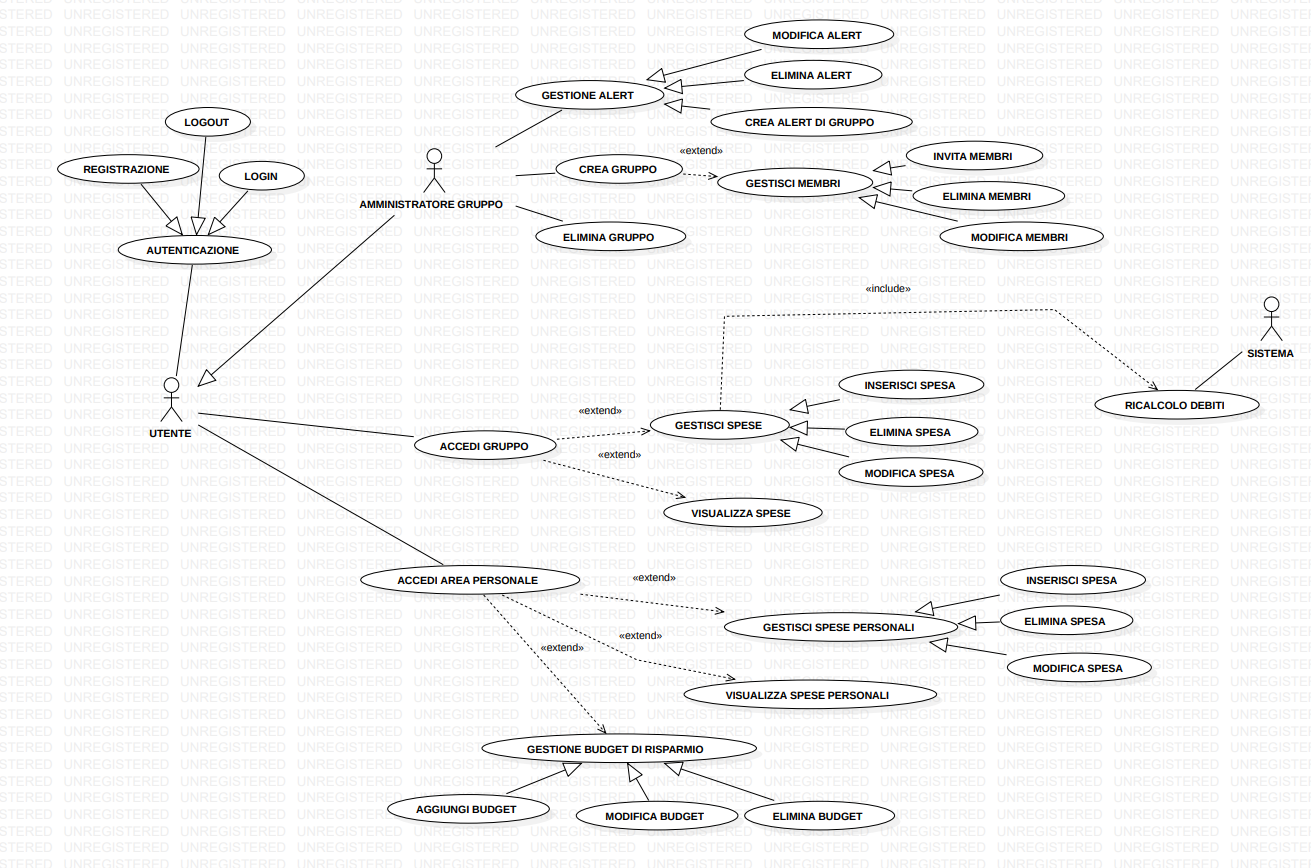
\includegraphics[scale=0.65]{C:/Users/loris/OneDrive/Desktop/PACproject/Documentazione/images/casousoprova.png}
        \caption{Diagramma casi d'uso }
    \end{figure}
Di seguito sono riportati alcuni casi d'uso principali:
\begin{itemize}
    \item \textbf{UC1 - Login}: Come utente, voglio poter accedere al mio account per gestire le mie spese.
    \item \textbf{UC2 - Registrazione}: Come nuovo utente, voglio potermi registrare al sistema per iniziare a usare la web-app.
    \item \textbf{UC3 - Logout}: Voglio poter terminare la mia sessione.
    \item \textbf{UC4 - Crea alert di gruppo}: Come utente amministratore di un gruppo spesa voglio poter inserire un alert, dove un alert è un avviso che ci permette di avvisare se si sta raggiungendo una soglia limite di spesa.
    \item \textbf{UC5 - Modifica alert}: Voglio poter modificare i valori dell'alert.
    \item \textbf{UC6 - Elimina alert}: Voglio poter eliminare l'alert. 
    \item \textbf{UC7 - Crea gruppo}: Voglio poter creare un gruppo di condivisione spese. 
    \item \textbf{UC8 - Invita memebri}: Voglio come amministratore invitare membri nel gruppo di spese.
    \item \textbf{UC9 - Elimina membri}: Voglio come amministratore poter eliminare membri del gruppo di spese.
    \item \textbf{UC10 - Modifica membri}: Voglio come amministratore modificare i membri nel gruppo di spese.
    \item \textbf{UC11 - Elimina gruppo}: Voglio poter eliminare un gruppo di condivisione spese. 
    \item \textbf{UC12 - Accedi gruppo}: Voglio poter accedere ad un gruppo di condivisione spese. 
    \item \textbf{UC13 - Inserisci spesa}: Voglio poter inserire una spesa di gruppo.
    \item \textbf{UC14 - Elimina spesa}: Voglio poter eliminare una spesa di gruppo.
    \item \textbf{UC15 - Modifica spesa}: Voglio poter modificare una spesa di gruppo.
    \item \textbf{UC16 - Visualizza spese}: Voglio poter visualizzare le spesa di gruppo.
    \item \textbf{UC17 - Ricalcolo debiti}: Voglio poter calcolare i debiti.
    \item \textbf{UC18 - Inserisci spesa personale}: Voglio poter inserire una spesa personali.
    \item \textbf{UC19 - Elimina spesa personale}: Voglio poter eliminare una spesa personali.
    \item \textbf{UC20 - Modifica spesa personale}: Voglio poter modificare una spesa personali.
    \item \textbf{UC21 - Visualizza spesa personale}: Voglio poter visualizzare le spesa personali.
    \item \textbf{UC22 - Inserisci budget}: Voglio poter inserire un budget di risparmio.
    \item \textbf{UC23 - Elimina budget}: Voglio poter eliminare un budget di risparmio.
    \item \textbf{UC24 - Modifica budget}: Voglio poter modificare un budget di risparmio.
    \item \textbf{UC25 - Visualizza budget}: Voglio poter visualizzare i budget di risparmio.
\end{itemize}

\section{Priorità casi d'uso}
    I casi d'uso possono essere suddivisi in tre categorie, a seconda della loro priorità nel processo di sviluppo:
    \begin{itemize}
        \item \textbf{Coda ad alta priorità:} 
        Contiene i requisiti essenziali per il corretto funzionamento dell'applicativo. Questi includono la creazione dei profili utente, la creazione di nuovi gruppi spese, con le funzionalità annesse(invita,elimina membri ecc ecc) ed infine la gestione spesa con l'algoritmo di calcolo debiti.
    
        \item \textbf{Coda a media priorità:} 
        Questa coda include funzionalità di supporto, principalmente orientate alla gestione spese personali.
    
        \item \textbf{Coda a bassa priorità:} 
        Contiene le funzionalità meno rilevanti ossia la tematica del budget , per le quali non è prevista una loro implementazione immediata. Tuttavia, potrebbero essere implementate in futuro, a seconda dell'andamento del progetto.
    \end{itemize}

    \begin{table}[h]
        \centering
        \begin{tabular}{|c|l|}
        \hline
        \textbf{ID} & \textbf{Titolo} \\ \hline
        UC1 & Login\\ \hline
        UC2 & Registrazione \\ \hline
        UC3 & Logout \\ \hline
        UC8 & Invita memebri \\ \hline
        UC9 & Elimina membri \\ \hline
        UC10 & Modica memebri \\ \hline
        UC11 & Elimina gruppo \\ \hline
        UC12 & Accedi gruppo \\ \hline
        UC13 & Inserisci spesa \\ \hline
        UC14 & Elimina spesa \\ \hline
        UC15 & Modifica spese \\ \hline
        UC16 & Visualizza spese \\ \hline
        UC17 & Ricalcolo debiti \\ \hline
        \end{tabular}
        \caption{Coda alta priorità}
    \end{table}

    \begin{table}[h]
        \centering
        \begin{tabular}{|c|l|}
        \hline
        \textbf{ID} & \textbf{Titolo} \\ \hline
        UC4 & Crea alert di gruppo\\ \hline
        UC5 & Modica alert \\ \hline
        UC6 & Elimina alert \\ \hline
        UC18 & Inserisci spesa personale \\ \hline
        UC19 & Elimina spesa personale \\ \hline
        UC20 & Modica spesa personale \\ \hline
        UC21 & Visualizza spesa personale \\ \hline
        \end{tabular}
        \caption{Coda media priorità}
    \end{table}

    \begin{table}[h]
        \centering
        \begin{tabular}{|c|l|}
        \hline
        \textbf{ID} & \textbf{Titolo} \\ \hline
        UC22 & Inserisci budget\\ \hline
        UC23 & Elimina budget \\ \hline
        UC24 & Modica budget \\ \hline
        UC25 & Visualizza budget \\ \hline
        \end{tabular}
        \caption{Coda media priorità}
    \end{table}


\section{Architettura}
    L'architettura del sistema è basata su un'architettura a microservizi con i seguenti componenti principali:
    \begin{itemize}
        \item \textbf{Client/Frontend}: Implementato in React.js, il frontend fornisce un'interfaccia utente intuitiva per la gestione delle spese.
        \item \textbf{API Gateway}: Un punto di ingresso unico per tutte le richieste del client, responsabile dell'instradamento verso i microservizi corretti.
        \item \textbf{Backend (Microservizi)}: I microservizi sono sviluppati in Spring Boot e includono:
        \begin{itemize}
            \item \textbf{Servizio Utente}: Gestisce la registrazione, l'autenticazione e il profilo utente.
            \item \textbf{Servizio Gestione Spese}: Gestisce le operazioni CRUD sulle spese.
            \item \textbf{Servizio Gruppi}: Gestisce la creazione e la modifica dei gruppi.
        \end{itemize}
        \item \textbf{Database}: Utilizzo di PostgreSQL per la gestione dei dati relazionali.
    \end{itemize}

\section{Toolchain}
Per la realizzazione della piattaforma \textbf{Spendly} verranno utilizzati i seguenti strumenti:

\subsection*{Modellazione}
\begin{itemize}
    \item Diagrammi (casi d'uso, deployment, componenti, classi, flussi, entità-relazione): \textbf{Draw.io}, \textbf{StarUML}.
\end{itemize}

\subsection*{Implementazione Applicazione Client}
\begin{itemize}
    \item Linguaggio di programmazione: \textbf{Java};
    \item IDE: \textbf{Visual Studio Code};
    \item Framework: \textbf{Spring}.
\end{itemize}

\subsection*{Implementazione Web Server}
\begin{itemize}
    \item Linguaggio di programmazione: \textbf{Java};
    \item IDE: \textbf{Visual Studio Code};
    \item Framework: \textbf{Spring};
    \item Analisi statica: \textbf{Checkstyle}, \textbf{SonarLint};
    \item Testing e analisi dinamica: \textbf{JUnit}.
\end{itemize}

\subsection*{Implementazione Database}
\begin{itemize}
    \item Tipologia: \textbf{Relazionale};
    \item Database: \textbf{MySQL};
    \item Gestione: \textbf{MySQL Workbench}.
\end{itemize}

\subsection*{Documentazione, Versioning e Organizzazione del Team}
\begin{itemize}
    \item Documentazione: \textbf{LaTeX};
    \item Versioning: \textbf{GitHub};
    \item Git Client: \textbf{GitHub Desktop};
    \item Organizzazione del Team: \textbf{Microsoft Teams}, \textbf{Trello}.
\end{itemize}
    